% Options for packages loaded elsewhere
\PassOptionsToPackage{unicode}{hyperref}
\PassOptionsToPackage{hyphens}{url}
\PassOptionsToPackage{dvipsnames,svgnames,x11names}{xcolor}
%
\documentclass[
  letterpaper,
  DIV=11,
  numbers=noendperiod]{scrartcl}

\usepackage{amsmath,amssymb}
\usepackage{iftex}
\ifPDFTeX
  \usepackage[T1]{fontenc}
  \usepackage[utf8]{inputenc}
  \usepackage{textcomp} % provide euro and other symbols
\else % if luatex or xetex
  \usepackage{unicode-math}
  \defaultfontfeatures{Scale=MatchLowercase}
  \defaultfontfeatures[\rmfamily]{Ligatures=TeX,Scale=1}
\fi
\usepackage{lmodern}
\ifPDFTeX\else  
    % xetex/luatex font selection
\fi
% Use upquote if available, for straight quotes in verbatim environments
\IfFileExists{upquote.sty}{\usepackage{upquote}}{}
\IfFileExists{microtype.sty}{% use microtype if available
  \usepackage[]{microtype}
  \UseMicrotypeSet[protrusion]{basicmath} % disable protrusion for tt fonts
}{}
\makeatletter
\@ifundefined{KOMAClassName}{% if non-KOMA class
  \IfFileExists{parskip.sty}{%
    \usepackage{parskip}
  }{% else
    \setlength{\parindent}{0pt}
    \setlength{\parskip}{6pt plus 2pt minus 1pt}}
}{% if KOMA class
  \KOMAoptions{parskip=half}}
\makeatother
\usepackage{xcolor}
\setlength{\emergencystretch}{3em} % prevent overfull lines
\setcounter{secnumdepth}{-\maxdimen} % remove section numbering
% Make \paragraph and \subparagraph free-standing
\makeatletter
\ifx\paragraph\undefined\else
  \let\oldparagraph\paragraph
  \renewcommand{\paragraph}{
    \@ifstar
      \xxxParagraphStar
      \xxxParagraphNoStar
  }
  \newcommand{\xxxParagraphStar}[1]{\oldparagraph*{#1}\mbox{}}
  \newcommand{\xxxParagraphNoStar}[1]{\oldparagraph{#1}\mbox{}}
\fi
\ifx\subparagraph\undefined\else
  \let\oldsubparagraph\subparagraph
  \renewcommand{\subparagraph}{
    \@ifstar
      \xxxSubParagraphStar
      \xxxSubParagraphNoStar
  }
  \newcommand{\xxxSubParagraphStar}[1]{\oldsubparagraph*{#1}\mbox{}}
  \newcommand{\xxxSubParagraphNoStar}[1]{\oldsubparagraph{#1}\mbox{}}
\fi
\makeatother


\providecommand{\tightlist}{%
  \setlength{\itemsep}{0pt}\setlength{\parskip}{0pt}}\usepackage{longtable,booktabs,array}
\usepackage{calc} % for calculating minipage widths
% Correct order of tables after \paragraph or \subparagraph
\usepackage{etoolbox}
\makeatletter
\patchcmd\longtable{\par}{\if@noskipsec\mbox{}\fi\par}{}{}
\makeatother
% Allow footnotes in longtable head/foot
\IfFileExists{footnotehyper.sty}{\usepackage{footnotehyper}}{\usepackage{footnote}}
\makesavenoteenv{longtable}
\usepackage{graphicx}
\makeatletter
\def\maxwidth{\ifdim\Gin@nat@width>\linewidth\linewidth\else\Gin@nat@width\fi}
\def\maxheight{\ifdim\Gin@nat@height>\textheight\textheight\else\Gin@nat@height\fi}
\makeatother
% Scale images if necessary, so that they will not overflow the page
% margins by default, and it is still possible to overwrite the defaults
% using explicit options in \includegraphics[width, height, ...]{}
\setkeys{Gin}{width=\maxwidth,height=\maxheight,keepaspectratio}
% Set default figure placement to htbp
\makeatletter
\def\fps@figure{htbp}
\makeatother

\usepackage{booktabs}
\usepackage{longtable}
\KOMAoption{captions}{tableheading}
\makeatletter
\@ifpackageloaded{caption}{}{\usepackage{caption}}
\AtBeginDocument{%
\ifdefined\contentsname
  \renewcommand*\contentsname{Table of contents}
\else
  \newcommand\contentsname{Table of contents}
\fi
\ifdefined\listfigurename
  \renewcommand*\listfigurename{List of Figures}
\else
  \newcommand\listfigurename{List of Figures}
\fi
\ifdefined\listtablename
  \renewcommand*\listtablename{List of Tables}
\else
  \newcommand\listtablename{List of Tables}
\fi
\ifdefined\figurename
  \renewcommand*\figurename{Figure}
\else
  \newcommand\figurename{Figure}
\fi
\ifdefined\tablename
  \renewcommand*\tablename{Table}
\else
  \newcommand\tablename{Table}
\fi
}
\@ifpackageloaded{float}{}{\usepackage{float}}
\floatstyle{ruled}
\@ifundefined{c@chapter}{\newfloat{codelisting}{h}{lop}}{\newfloat{codelisting}{h}{lop}[chapter]}
\floatname{codelisting}{Listing}
\newcommand*\listoflistings{\listof{codelisting}{List of Listings}}
\makeatother
\makeatletter
\makeatother
\makeatletter
\@ifpackageloaded{caption}{}{\usepackage{caption}}
\@ifpackageloaded{subcaption}{}{\usepackage{subcaption}}
\makeatother

\ifLuaTeX
  \usepackage{selnolig}  % disable illegal ligatures
\fi
\usepackage{bookmark}

\IfFileExists{xurl.sty}{\usepackage{xurl}}{} % add URL line breaks if available
\urlstyle{same} % disable monospaced font for URLs
\hypersetup{
  pdftitle={DAA with MAasLin 3},
  colorlinks=true,
  linkcolor={blue},
  filecolor={Maroon},
  citecolor={Blue},
  urlcolor={Blue},
  pdfcreator={LaTeX via pandoc}}


\title{DAA with MAasLin 3}
\author{}
\date{}

\begin{document}
\maketitle


\subsubsection{Differential abundance
analysis}\label{differential-abundance-analysis}

\begin{itemize}
\tightlist
\item
  Group variable: \textbf{diet}
\item
  Formula used: \textbf{\textasciitilde{} diet * time}
\end{itemize}

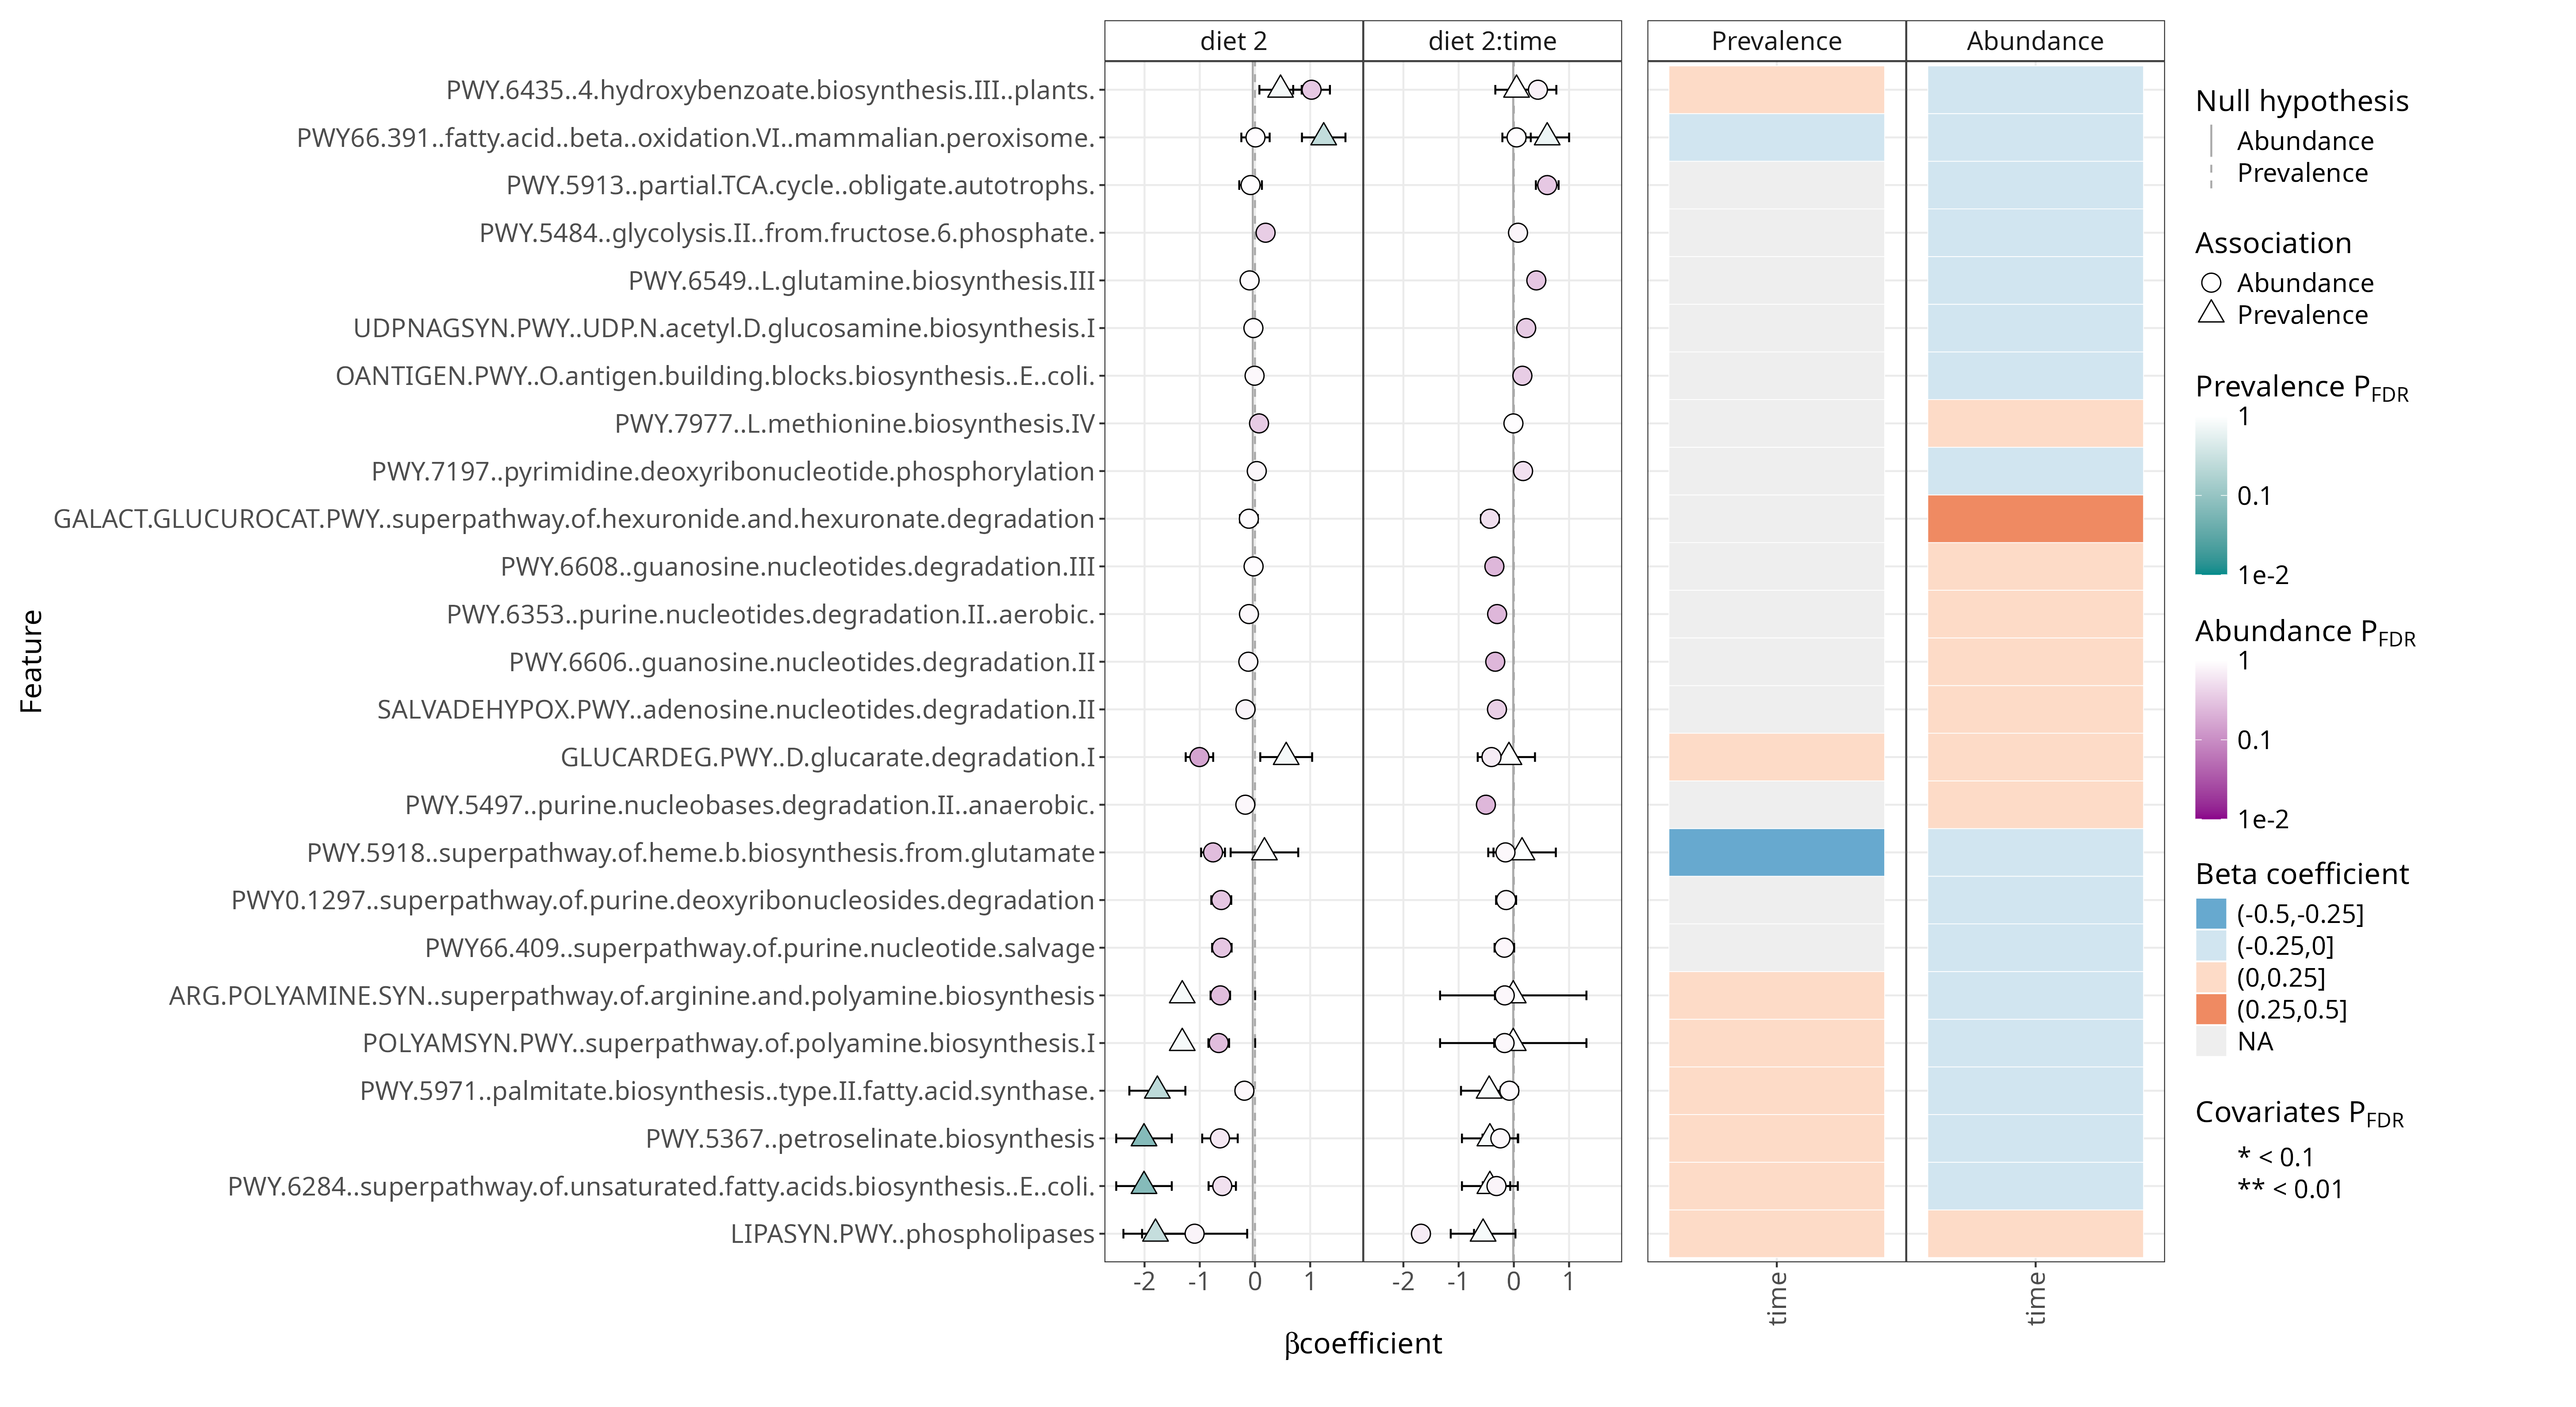
\includegraphics{../output/daa_maaslin3/figures/summary_plot.png}
\includegraphics{../output/daa_maaslin3/figures/association_plots/diet/linear/diet_ANAGLYCOLYSIS.PWY..glycolysis.III..from.glucose._linear.png}
\includegraphics{../output/daa_maaslin3/figures/association_plots/diet/linear/diet_ARG.POLYAMINE.SYN..superpathway.of.arginine.and.polyamine.biosynthesis_linear.png}
\includegraphics{../output/daa_maaslin3/figures/association_plots/diet/linear/diet_ARO.PWY..chorismate.biosynthesis.I_linear.png}
\includegraphics{../output/daa_maaslin3/figures/association_plots/diet/linear/diet_BRANCHED.CHAIN.AA.SYN.PWY..superpathway.of.branched.chain.amino.acid.biosynthesis_linear.png}
\includegraphics{../output/daa_maaslin3/figures/association_plots/diet/linear/diet_CALVIN.PWY..Calvin.Benson.Bassham.cycle_linear.png}
\includegraphics{../output/daa_maaslin3/figures/association_plots/diet/linear/diet_COA.PWY..coenzyme.A.biosynthesis.I..prokaryotic._linear.png}
\includegraphics{../output/daa_maaslin3/figures/association_plots/diet/linear/diet_COA.PWY.1..superpathway.of.coenzyme.A.biosynthesis.III..mammals._linear.png}
\includegraphics{../output/daa_maaslin3/figures/association_plots/diet/linear/diet_COLANSYN.PWY..colanic.acid.building.blocks.biosynthesis_linear.png}
\includegraphics{../output/daa_maaslin3/figures/association_plots/diet/linear/diet_COMPLETE.ARO.PWY..superpathway.of.aromatic.amino.acid.biosynthesis_linear.png}
\includegraphics{../output/daa_maaslin3/figures/association_plots/diet/linear/diet_DTDPRHAMSYN.PWY..dTDP..beta..L.rhamnose.biosynthesis_linear.png}
\includegraphics{../output/daa_maaslin3/figures/association_plots/diet/linear/diet_GLUCARDEG.PWY..D.glucarate.degradation.I_linear.png}
\includegraphics{../output/daa_maaslin3/figures/association_plots/diet/linear/diet_HISTSYN.PWY..L.histidine.biosynthesis_linear.png}
\includegraphics{../output/daa_maaslin3/figures/association_plots/diet/linear/diet_ILEUSYN.PWY..L.isoleucine.biosynthesis.I..from.threonine._linear.png}
\includegraphics{../output/daa_maaslin3/figures/association_plots/diet/linear/diet_NONMEVIPP.PWY..methylerythritol.phosphate.pathway.I_linear.png}
\includegraphics{../output/daa_maaslin3/figures/association_plots/diet/linear/diet_OANTIGEN.PWY..O.antigen.building.blocks.biosynthesis..E..coli._linear.png}
\includegraphics{../output/daa_maaslin3/figures/association_plots/diet/linear/diet_PANTO.PWY..phosphopantothenate.biosynthesis.I.g__Alistipes.s__Alistipes_finegoldii_linear.png}
\includegraphics{../output/daa_maaslin3/figures/association_plots/diet/linear/diet_PEPTIDOGLYCANSYN.PWY..peptidoglycan.biosynthesis.I..meso.diaminopimelate.containing._linear.png}
\includegraphics{../output/daa_maaslin3/figures/association_plots/diet/linear/diet_PWY.1042..glycolysis.IV_linear.png}
\includegraphics{../output/daa_maaslin3/figures/association_plots/diet/linear/diet_PWY.2942..L.lysine.biosynthesis.III_linear.png}
\includegraphics{../output/daa_maaslin3/figures/association_plots/diet/linear/diet_PWY.3001..superpathway.of.L.isoleucine.biosynthesis.I_linear.png}
\includegraphics{../output/daa_maaslin3/figures/association_plots/diet/linear/diet_PWY.3001..superpathway.of.L.isoleucine.biosynthesis.I.g__Blautia.s__Ruminococcus_torques_linear.png}
\includegraphics{../output/daa_maaslin3/figures/association_plots/diet/linear/diet_PWY.3841..folate.transformations.II..plants._linear.png}
\includegraphics{../output/daa_maaslin3/figures/association_plots/diet/linear/diet_PWY.5097..L.lysine.biosynthesis.VI_linear.png}
\includegraphics{../output/daa_maaslin3/figures/association_plots/diet/linear/diet_PWY.5097..L.lysine.biosynthesis.VI.g__Blautia.s__Ruminococcus_torques_linear.png}
\includegraphics{../output/daa_maaslin3/figures/association_plots/diet/linear/diet_PWY.5103..L.isoleucine.biosynthesis.III_linear.png}
\includegraphics{../output/daa_maaslin3/figures/association_plots/diet/linear/diet_PWY.5130..2.oxobutanoate.degradation.I.unclassified_linear.png}
\includegraphics{../output/daa_maaslin3/figures/association_plots/diet/linear/diet_PWY.5686..UMP.biosynthesis.I_linear.png}
\includegraphics{../output/daa_maaslin3/figures/association_plots/diet/linear/diet_PWY.5941..glycogen.degradation.II.g__Blautia.s__Ruminococcus_torques_linear.png}
\includegraphics{../output/daa_maaslin3/figures/association_plots/diet/linear/diet_PWY.6121..5.aminoimidazole.ribonucleotide.biosynthesis.I_linear.png}
\includegraphics{../output/daa_maaslin3/figures/association_plots/diet/linear/diet_PWY.6122..5.aminoimidazole.ribonucleotide.biosynthesis.II_linear.png}
\includegraphics{../output/daa_maaslin3/figures/association_plots/diet/linear/diet_PWY.6123..inosine.5..phosphate.biosynthesis.I_linear.png}
\includegraphics{../output/daa_maaslin3/figures/association_plots/diet/linear/diet_PWY.6124..inosine.5..phosphate.biosynthesis.II_linear.png}




\end{document}
